\subsection{Architecture et fonctionnement}

HBase est un SGBD distribué et en tant que tel, il s'installe sur un cluster d'ordinateurs. Comme Hadoop, HBase s'installe sur un cluster en architecture Maître/Esclave. Dans la terminologie HBase, le nœud maître s'appelle le HMaster, et les nœuds esclaves s'appellent les RegionsServers. Le stockage des données est distribué sur les RegionsServers qui sont gérés par le HMaster. Le HMaster gère les métadonnées des tables HBase et coordonne l'exécution des activités des RegionsServers, tandis que les RegionsServers effectuent les opérations de lecture/écriture de données dans le cluster. La gestion du volume de données se fait par l'ajout des RegionsServers supplémentaires dans le cluster. La figure ci-après illustre l'architecture d'un cluster HBase.

\begin{figure}[h]
	\centering
    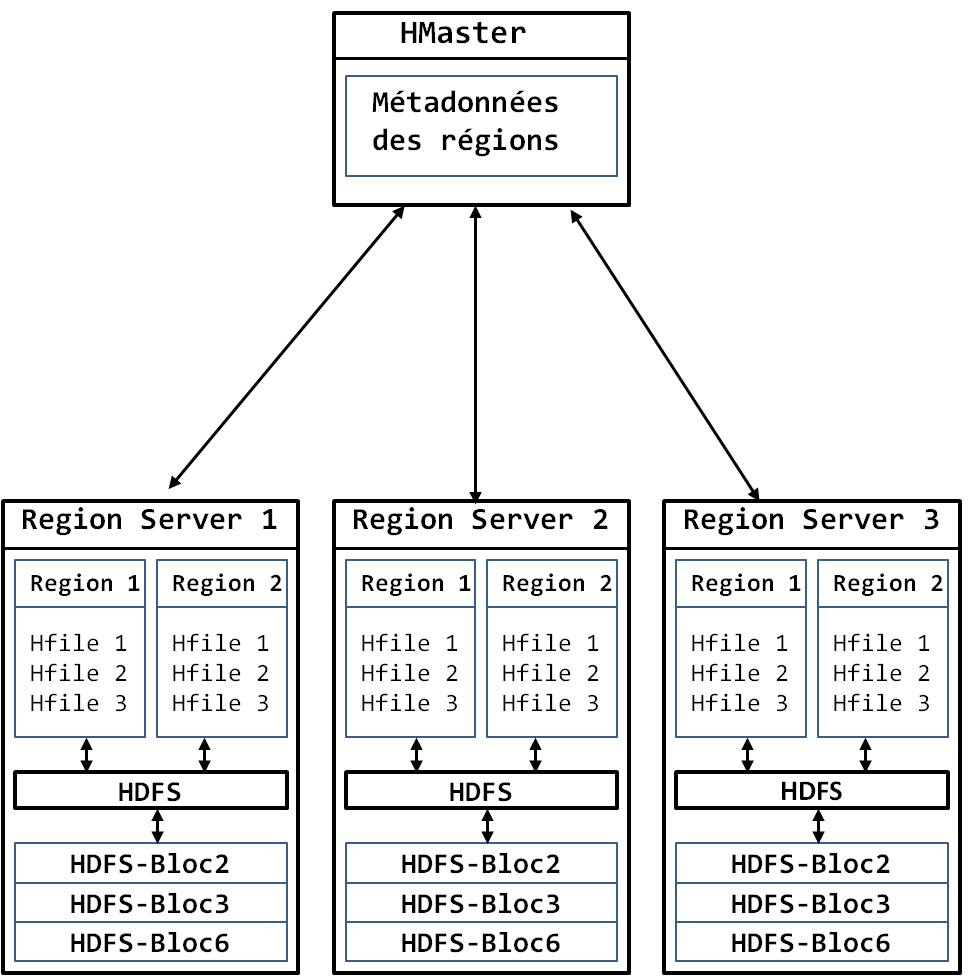
\includegraphics[scale=0.7]{img/part2/2.2}
    \caption{Architecture d'un cluster HBase.}
\end{figure}

\newpage
Comme vous le savez déjà, les tables HBase sont persistées sur le disque sous forme de fichiers HDFS appelés HFiles. Chaque HFile contient les données d'une et une seule famille de colonnes. Toutes les lignes de la table sont identifiées de façon unique à l'aide d'une valeur de la row key. Étant donné que la table fait office de base de données, pour une application métier donnée, toutes les données sont stockées dans la seule table HBase, qui pourra alors rapidement contenir des milliards de lignes, chiffrant sa taille en Téra octets voir Péta-octets. Cette taille phénoménale rend impossible le stockage de la table sur une seule machine. Pour résoudre ce problème, les tables HBase sont divisées en partitions appelées "régions" qui sont réparties entre les nœuds RegionsServers pour le stockage. La taille de chaque région peut être paramétrée dans un fichier de configuration hbase-site.xml. Lorsque la taille d'une région dépasse la taille maximale que vous avez définie dans le fichier de configuration, la région se partitionne automatiquement en deux. La région est une partition de la table triée par valeurs de la row key. La table étant déjà physiquement partitionné en HFiles, une région sera physiquement persistée sous forme d'un ou plusieurs HFiles. Les régions forment l'unité de stockage en HBase et sont la clé de la distribution du stockage et de la scalabilité du cluster HBase. La figure suivante illustre la façon dont HBase partitionne les tables en régions.

\begin{figure}[h]
	\centering
    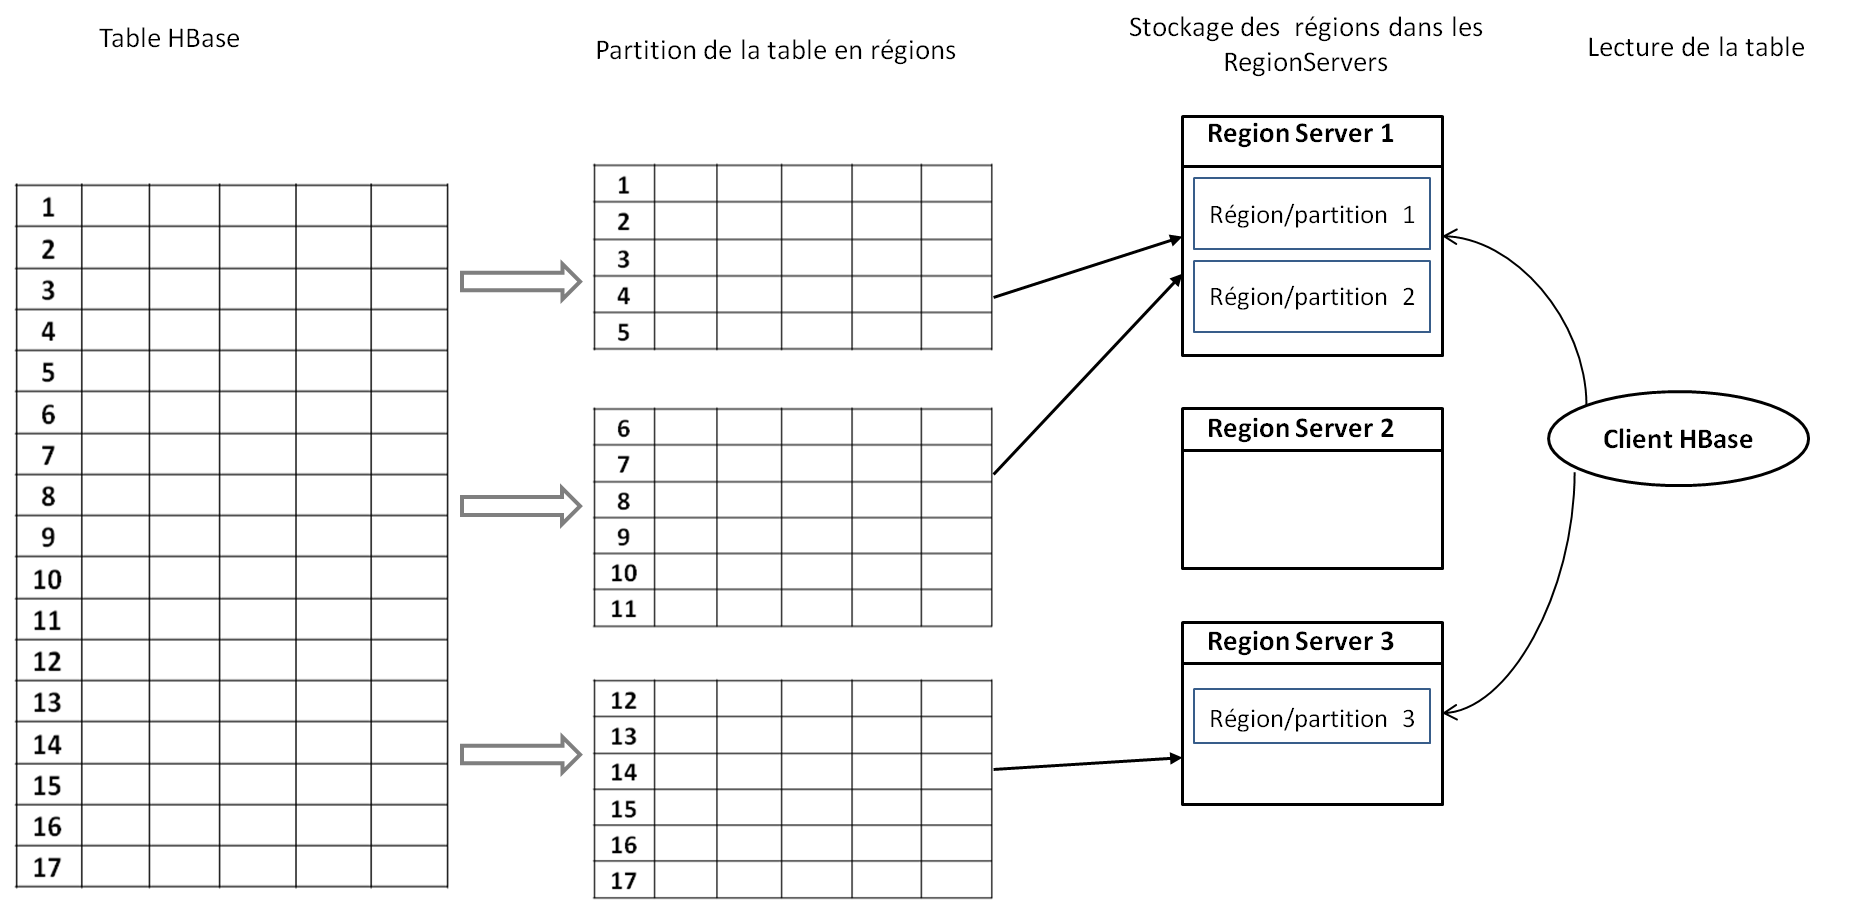
\includegraphics[scale=0.5]{img/part2/2.3}
    \caption{Partition des tables HBase.}
\end{figure}

\newpage
Les régions sont distribuées sur le cluster de façon aléatoire et chaque nœud RegionsServer peut stocker une ou plusieurs régions. Celle-ci sont répliquées entre les nœuds de façon à maintenir la disponibilité du cluster en cas de panne. Lors de l'ajout d'une ligne existante dans une table (nouvelle version de la ligne), HBase retrouve la région contenant la valeur de la row key de la ligne et l'insère dans cette région. Pour retrouver la région contenant la row key, HBase utilise une table de catalogue spéciale appelée "hbase:META". Cette table contient la liste des RegionsServers disponibles, et la liste des intervalles de valeurs de row key pour chaque région de table. Elle est stockée dans un composant de l'écosystème Hadoop appelé ZooKeeper, qui tourne sur un cluster différent du cluster sur lequel est installé Hbase. ZooKeeper est nécessaire parce qu'à la différence d'Hadoop où la communication entre le client et le cluster se fait à l'intermédiaire du nœud de référence, dans HBase, le client communique directement avec les nœuds RegionsServer sans passer par le HMaster. Le client n'a donc aucun moyen de connaître dans quel RegionsServer sont situées les données dont il a besoin. Lorsqu'un client fait une requête sur une row key précise, ZooKeeper pointe vers la table hbase : META pour récupérer les informations de la région contenant la row key, ensuite ZooKeeper renvoie cette information au client, qui va alors directement s'adresser au RegionsServer contenant la région. Finalement, la RegionsServer va traiter la requête et renvoyer au client les données de la row key.  La figure ci-après illustre le fonctionnement d'HBase lors d'une opération de lecture de données.

\begin{figure}[h]
	\centering
    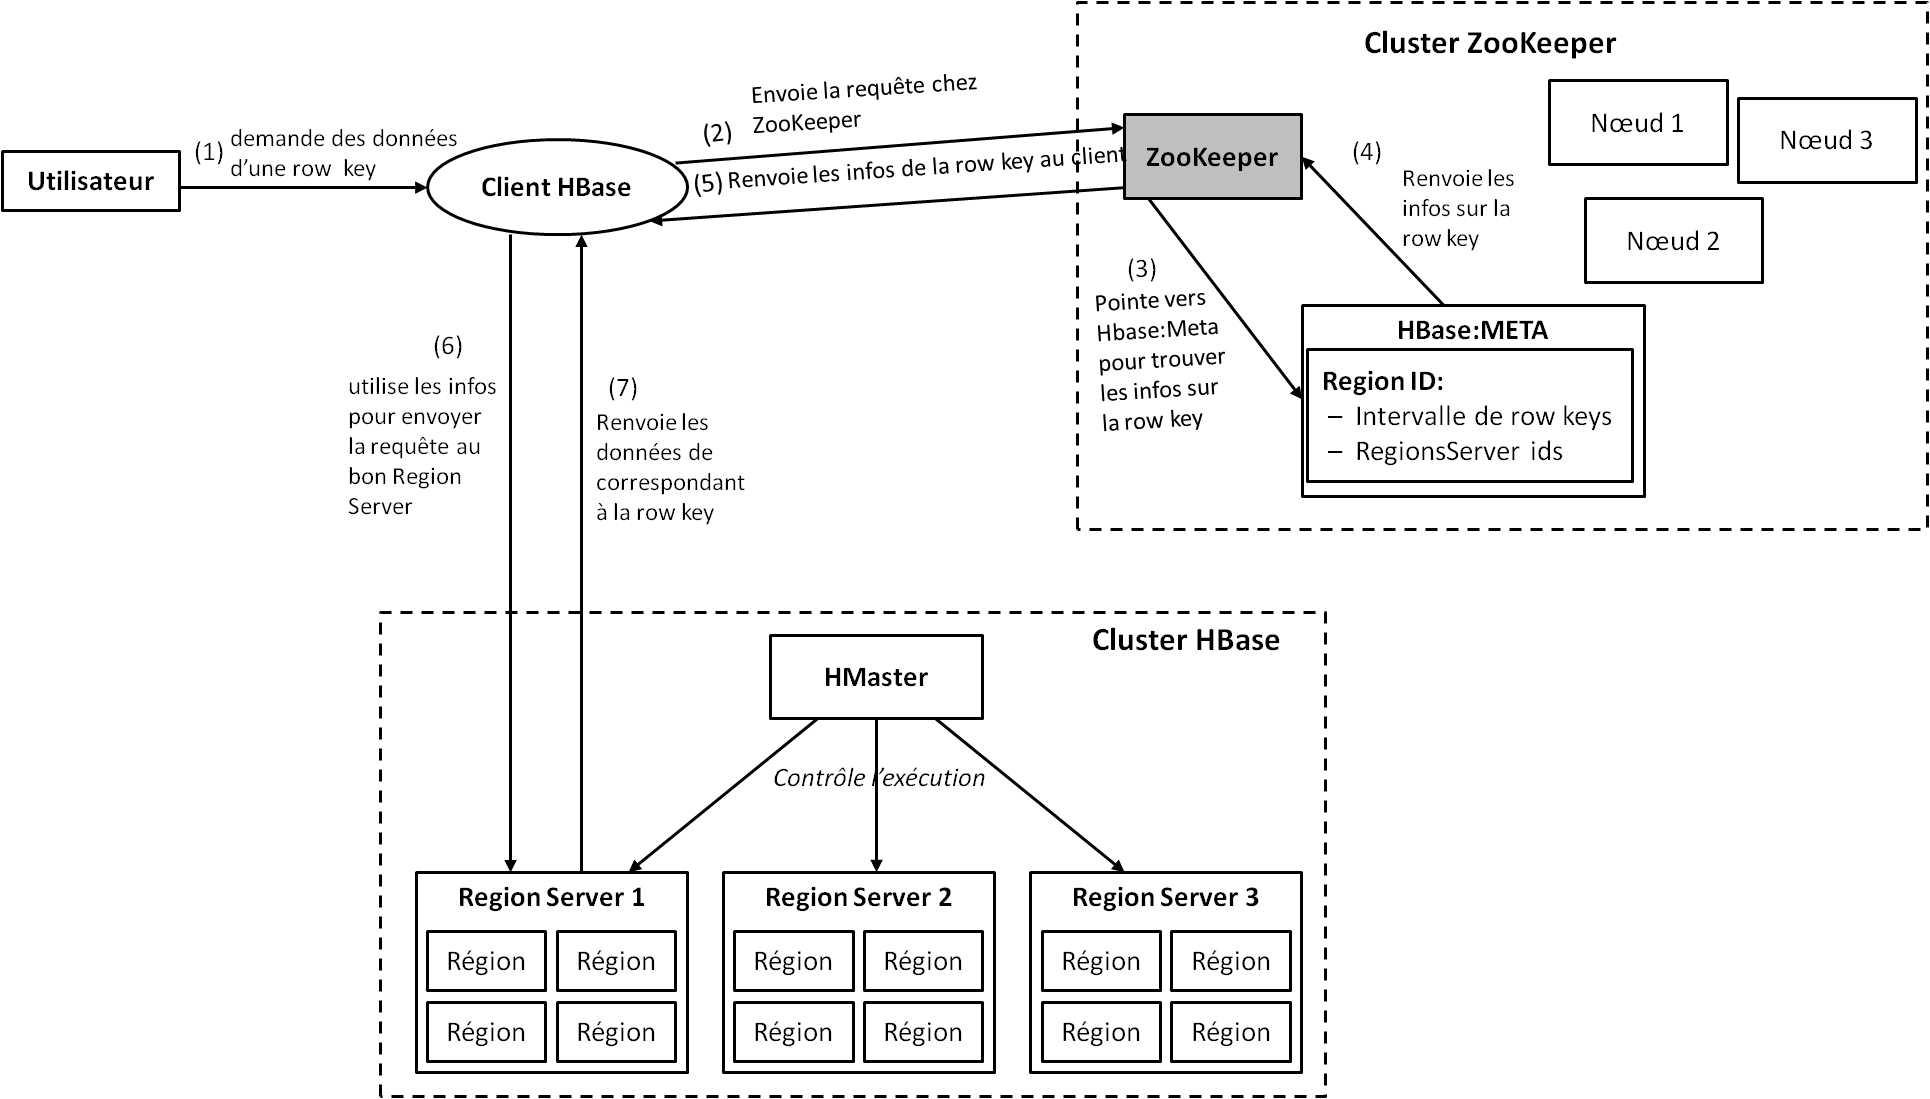
\includegraphics[scale=0.4]{img/part2/2.4}
    \caption{Fonctionnement de HBase.}
\end{figure}

\textit{\textbf{Remarque: }Ce mode de fonctionnement est effectif uniquement à partir de la version 0.96 d'HBase. Antérieurement à cette version, HBase utilisait deux tables de catalogue pour gérer les références de régions : .META. et –ROOT-. .META. contenaient la liste des RegionsServers disponibles, la liste des partitions dans chaque RegionsServer et leurs valeurs de row key. .META. était partitionnée en régions et lorsqu'un client envoyait une requête sur une row key précise, la requête n'accédait pas directement à la table .META., mais elle accédait à la table -ROOT-. La table -ROOT- était gérée par ZooKeeper et pointait vers la liste des régions .META. À partir de la version 0.96, la table –ROOT- a été supprimée et la table .META. a été remplacée par la table hbase:META actuelle. La table  hbase:META n'est désormais plus gérée par HBase, mais par ZooKeeper.}














